%\documentclass{beamer}
%Для защит онлайн лучше использовать разрешение 16x9
\documentclass[aspectratio=169]{beamer}

%%% Обязательные пакеты
%% Beamer
\usepackage{beamerthemesplit}
\usetheme{SPbGU}
\beamertemplatenavigationsymbolsempty
\usepackage{appendixnumberbeamer}

%% Локализация
\usepackage{fontspec}
\setmainfont{CMU Serif}
\setsansfont{CMU Sans Serif}
\setmonofont{CMU Typewriter Text}
%\setmonofont{Fira Code}[Contextuals=Alternate,Scale=0.9]
%\setmonofont{Inconsolata}
% \newfontfamily\cyrillicfont{CMU Serif}

\usepackage{polyglossia}
\setdefaultlanguage{russian}
\setotherlanguage{english}
\usepackage[autostyle]{csquotes} % Правильные кавычки в зависимости от языка

%% Графика
\usepackage{wrapfig} % Позволяет вставлять графику, обтекаемую текстом
\usepackage{pdfpages} % Позволяет вставлять многостраничные pdf документы в текст

%% Математика
\usepackage{amsmath, amsfonts, amssymb, amsthm, mathtools} % "Адекватная" работа с математикой в LaTeX

% Математические окружения с русским названием
\newtheorem{rutheorem}{Теорема}
\newtheorem{ruproof}{Доказательство}
\newtheorem{rudefinition}{Определение}
\newtheorem{rulemma}{Лемма}


%%% Дополнительные пакеты. Используются в презентации, но могут быть отключены при необходимости
\usepackage{tikz} % Мощный пакет для создание рисунков, однако может очень сильно замедлять компиляцию
\usetikzlibrary{decorations.pathreplacing,calc,shapes,positioning,tikzmark}

\usepackage{multirow} % Ячейка занимающая несколько строк в таблице

%% Пакеты для оформления алгоритмов на псевдокоде
\usepackage[noend]{algpseudocode}
\usepackage{algorithm}
\usepackage{algorithmicx}

\usepackage{fancyvrb}

%% Пакет для анимированных иллюстраций
\usepackage{animate}


% То, что в квадратных скобках, отображается внизу по центру каждого слайда. 
\title[Улучшение производительности RPQ]
{Улучшение производительности алгоритма достижимости с регулярными ограничениями на графическом ускорителе}

% То, что в квадратных скобках, отображается в левом нижнем углу. 
\institute[СПбГУ]{}

% То, что в квадратных скобках, отображается в левом нижнем углу.
\author[Дмитрий Козенко]{Козенко Дмитрий Сергеевич, группа 23.Б08-мм}
 
\begin{document}
{
\setbeamertemplate{footline}{}
% Лого университета или организации, отображается в шапке титульного листа
\begin{frame}
  
\includegraphics[width=1.4cm]{pictures/SPbGU_Logo.png}
\vspace{-35pt}
\hspace{-10pt}
\begin{center}
   \begin{tabular}{c}
        \scriptsize{Санкт-Петербургский государственный университет} \\
        \scriptsize{Кафедра системного программирования}
    \end{tabular}
\titlepage
\end{center}

\btVFill

{\scriptsize
  % У научного руководителя должна быть указана научная степень
   \textbf{Научный руководитель:} к.ф.-м.н. С.В. Григорьев, доцент кафедры системного программирования
 }
\begin{center}
  \vspace{5pt}
  \scriptsize{Санкт-Петербург\\2025}
  \end{center}
\end{frame}
}

\begin{frame}[fragile]  
  \frametitle{Графовые базы данных и запросы с регулярными ограничениями}
  \begin{itemize}
    \item Запросы с регулярными ограничениями активно используются в графовых базах данных
    \item Алгоритм RPQ\footnote{RPQ с линейной алгеброй: \url{https://se.math.spbu.ru/thesis/texts/Beljanin_Georgij_Olegovich_Spring_practice_2nd_year_2024_text.pdf}  (Дата доступа: 19.06.2025)} основан на операциях линейной алгебры, которые отлично подходят вычислений на GPU
    \item Текущая реализация RPQ\footnote{GitHub репозитория с реализацией алгоритма на GPU: \url{https://github.com/mitya-y/rpq/tree/cb2583e} (Дата доступа: 19.06.2025)} на GPU на наборе данных Wikidata проигрывает CPU почти в 4 раза
  \end{itemize}
\end{frame}

% Обязательный слайд: четкая формулировка цели данной работы и постановка задачи
% Описание выносимых на защиту результатов, процесса или особенностей их достижения и т.д.
\begin{frame}
  \frametitle{Постановка задачи}

\textbf{Целью} работы является анализ узких мест реализации алгоритма на GPU и улучшение еe производительности

\textbf{Задачи}:
\begin{enumerate}
    \item Воспроизвести тестирование из прошлой работы, проанализировать результаты и найти узкие места алгоритма
    \item Улучшить производительность алгоритма
    \item Провести эксперименты c итоговой версией алгоритма
    \item Перенести свою ветку update-cuda-12.6 в основной репозиторий cuBool, организовать репозиторий с алгоритмами, использующими cuBool, и добавить в нее свой алгоритм
\end{enumerate}
\end{frame}

\begin{frame}
  \frametitle{Описание данных и стендов}
В ходе работы над анализом алгоритма были проведены измерения на следующих наборах данных
\begin{itemize}
    \item Wikidata\footnote{База знаний WikiData: \href{https://www.wikidata.org/wiki/Wikidata:Database_download}{https://www.wikidata.org/wiki/Wikidata:Database\_download} (Дата доступа 19.06.25)}: набор данных из реального мира вместе с 660 запросами
    \item RPQ-Bench\footnote{Набор данных RPQ-Bench: \url{https://github.com/Mamenglu/LD-RPQB} (Дата доступа 19.06.25)}: синтетический набор данных, 20 типов запросов. Было создано 2 датасета: c графом на $10^7$ вершин, по 1000 запросов каждого типа и с графом на $10^8$ вершин и 100 запросов каждого вида
\end{itemize}

Были использованы следующие тестовые стенды
\begin{itemize}
    \item Intel i5-10400f и Nvidia RTX 3050 (8 Gb VRAM), 16 Gb RAM, Manjaro 6.14
    \item AMD Ryzen 9 7900X и Nvidia RTX 3090 (24 Gb VRAM), 128 Gb RAM, Ubuntu 24.04
\end{itemize}

\end{frame}
 
\begin{frame}
  \frametitle{Улучшение алгоритма}
Для улучшения производительности алгоритма были применены следующие изменения:
\begin{enumerate}
    \item Изменена реализация функции сложения матриц --- используется схожая поэлементному умножению матриц реализация вместо библиотеки Nsparse
    \item Исправлена ошибка в cmake с конфигурациями сборки
    \item Добавлена возможно передавать транспонированные матрицы в алгоритм
\end{enumerate}

\begin{table}[]
    \caption{Сравнение времени работы алгоритма до и после изменений}
    \centering
    \scalebox{0.9}{
        \begin{tabular}{|c|с|c|}
            \hline
            \makecell{Версия \\ алгоритма} & 
            \makecell{Время выполнения \\ 520 запросов, c} & 
            \makecell{Время \\ загрузки, c} \\
            \hline
            Без изменений & 273.09 & 5704.66 \\
            \hline
            С изменениями & 84.61 & 666.15 \\
            \hline
        \end{tabular}
    }
\end{table}

\end{frame}

\begin{frame}
    \frametitle{Организация репозитория cuBoolGraph\footnote{GitHub репозиторий cuBoolGraph: \url{https://github.com/SparseLinearAlgebra/cuBoolGraph} (Дата доступа: 19.06.2025)}}

\begin{figure}
    \centering
    % 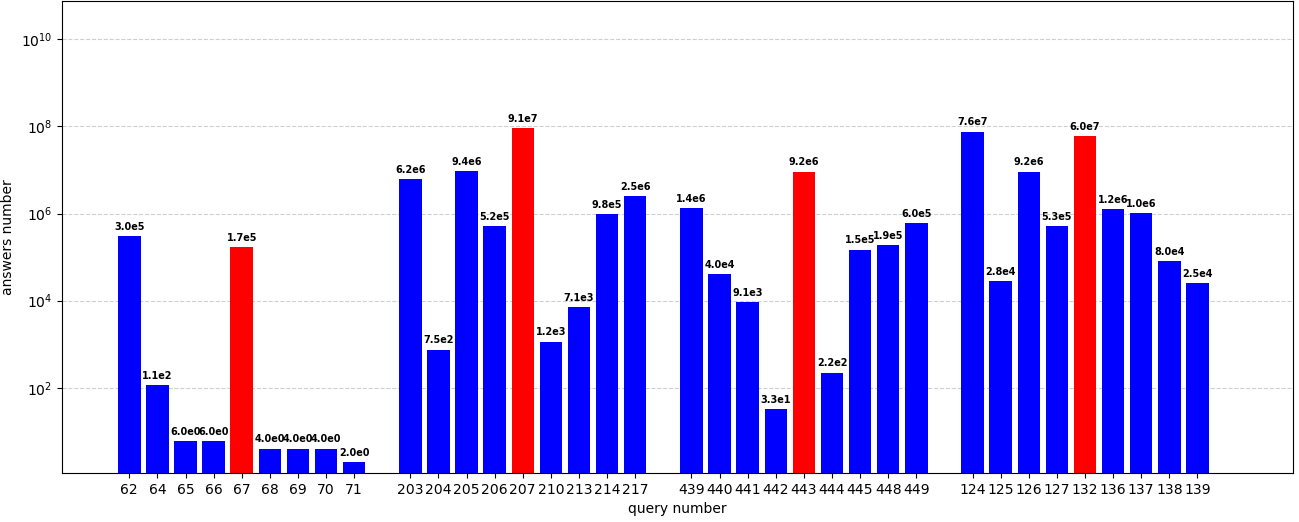
\includegraphics[width=\textwidth]{figures/answers_scaled.png}
    % 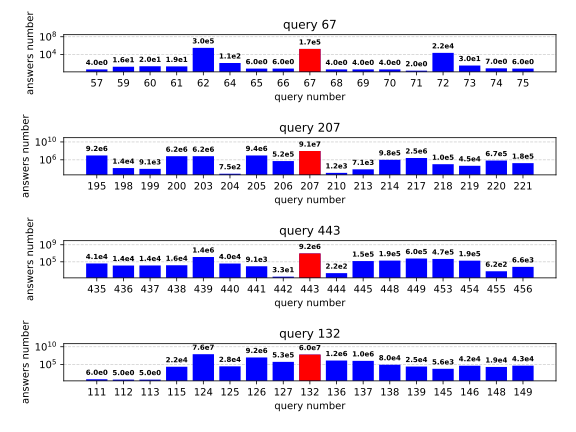
\includegraphics[scale = 0.36]{figures/worst.png}
    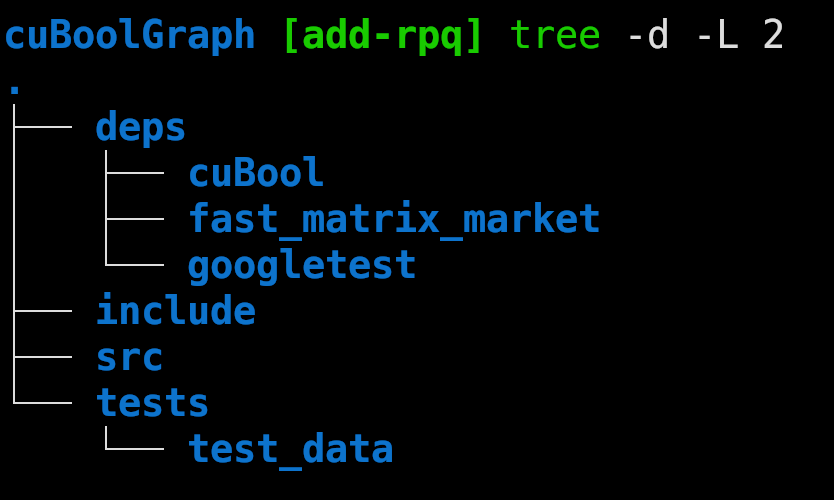
\includegraphics[scale = 0.36]{pictures/cuBoolGraph.png}
    \caption{Структура репозитория cuBoolGraph}
    \label{fig:cuBoolGraph}
\end{figure}

\end{frame}
 
\begin{frame}[t]
  \frametitle{Эксперимент}
Для дальнейшего анализа производительности алгоритма были поставлены следующие задачи
\begin{enumerate}
    \item Замерить время работы реализаций на CPU и GPU и проанализировать типы запросов, работающих на GPU медленее, чем на CPU
    \item Изучить масштабируемость реализации для GPU, сравнив время работы на двух разных по мощности тестовых стендах
\end{enumerate}  

Суммарное время работы выполнения всех запросов:
\begin{table}
    \centering
    \begin{tabular}{|c|c|c|c|}
\hline
Данные & Время GPU, \si{\second} & Время CPU, \si{\second} & Ускорение GPU \\
\hline
Wikidata & 115.73 & 136.30 & 1.18 \\
\hline
RPQ-bench $10^7$ & 185.28 & 55.19 & 0.30 \\
\hline
    \end{tabular}
    \caption{Результаты сравнения CPU и GPU}
    \label{tab:ExpResults}
\end{table}
\end{frame}

\begin{frame}[t]
  \frametitle{Анализ набора данных Wikidata}
  
\begin{figure}[H]
    \centering
    % 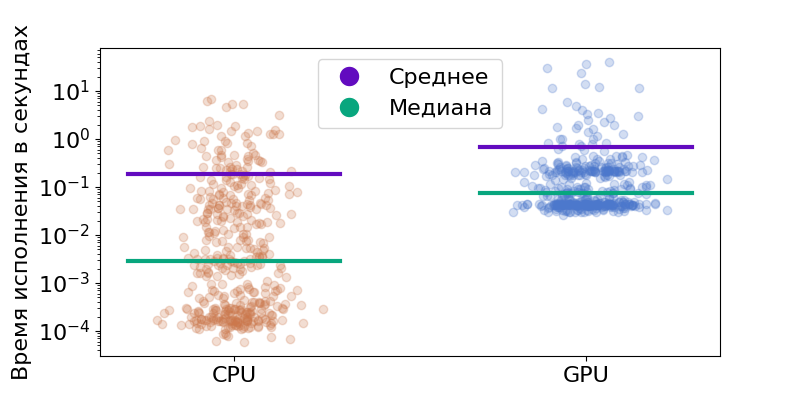
\includegraphics[scale = 0.57]{pictures/Cloud.png}
    \includesvg[width=\textheight, pretex=\small]{pictures/cloud.svg} 
    \caption{Облако распределения времени исполнения запросов}
    \label{GraphicFull}  
\end{figure}
    
\end{frame}


% \begin{frame}[t]
%   \frametitle{Анализ набора данных Wikidata}
% \begin{table}[ht]
% \centering
% \caption{4 запроса, на которых GPU сильно проигрывает}
% \label{tab:worst4queris}
% \scalebox{0.7}{
%     \begin{tabular}{|c|c|c|c|с|}
%     \hline
%     № запроса & Вид & {Замедление} & {Время GPU, s} & {Время CPU, s} \\
%     \hline
%     132  & $(a^*~b^*)^+$ & 1.58   & 11.28  & 7.16  \\
%     \hline
%     443  & $a^*$ & 2.27   & 2.61   & 1.15  \\
%     \hline
%     207  & $(a\mid b)^+$ & 2.52   & 17.34  & 6.88  \\
%     \hline
%     % 67   & $((\widehat{\phantom{c}}\: a)~a)+$ & 43.05  & 9.04   & 0.21  \\
%     67   & $(~\hat{}a~a)^+$ & 43.05  & 9.04   & 0.21  \\
%     \hline
%     \end{tabular}
% }
% \end{table}
%  
% \begin{figure}[H]
%     \centering
%     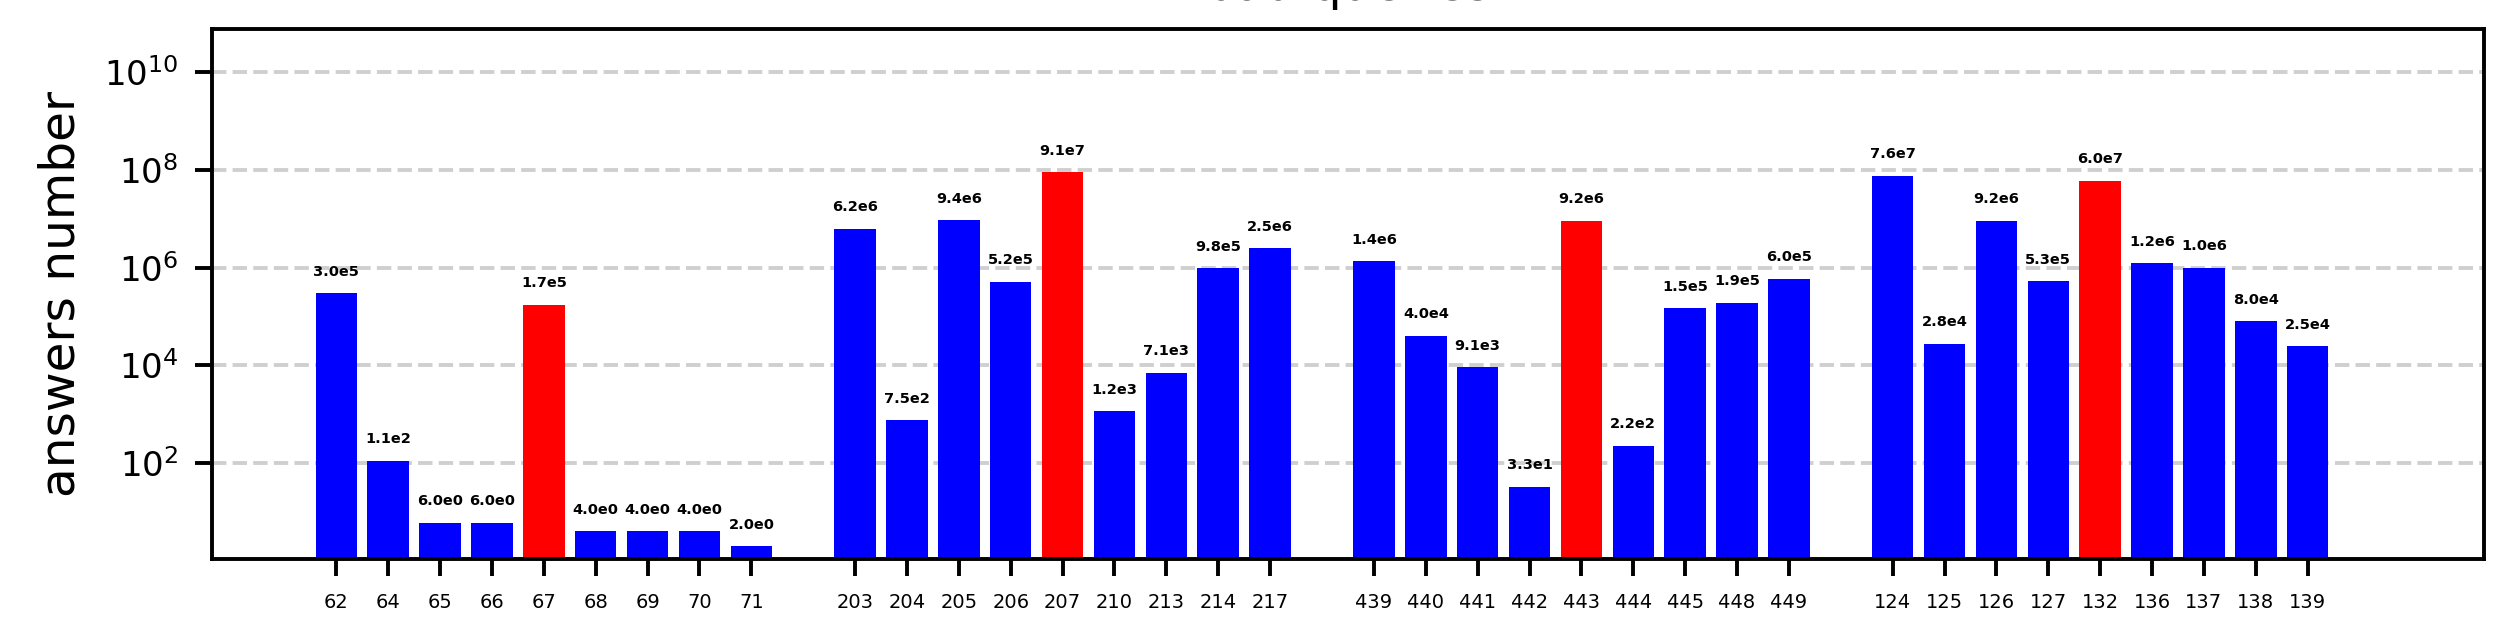
\includegraphics[scale = 0.13]{pictures/scaled_bads.png}
%     \caption{Анализ количества ответов}
% \end{figure}
%    
% \end{frame}

\begin{frame}[t]
  \frametitle{Анализ набора данных RPQ-bench}
 
\begin{table}[ht]
\centering
\caption{Время работы каждой операции на наборе данных RPQ-bench $10^7$ в реализациях на GPU и CPU}
\label{tab:RpqBenchVtune}
\scalebox{1.2}{
    \begin{tabular}{|l|c|c|}
    \hline
    Операция & GPU, s \si{\second} & CPU, s \si{\second} \\
    \hline
    \centering
    \texttt{MxM} & 177.66 (78.93\%) & 20.37 (37.13\%)  \\
    \texttt{VxM} & 26.16 (11.62\%) & 8.08 (14.73\%) \\
    \texttt{cuBool\_EwiseAdd} & 7.59 (3.37\%) & --- \\
    \texttt{cuBool\_EwiseMulInverted} & 12.90 (5.73\%) & --- \\
    \texttt{GrB\_Matrix\_assign} & --- & 26.22 (47.79\%) \\
    \hline
    \end{tabular}
}
\end{table}

\end{frame}

 
\begin{frame}[t]
  \frametitle{Анализ масштабируемости алгоритма}

% Для полной загрузки более мощной видеокарты был создан более крупный датасет RPQ-bench на $10^8$ вершин

Суммарное время работы выполнения всех запросов:
\begin{table}[ht]
\centering
\caption{Результаты замеров на RTX 3050 и RTX 3090}
\scalebox{0.7}{
    \begin{tabular}{|c|c|c|c|}
    \hline
    Набор данных & RTX 3050, s & RTX 3090, s & Ускорение \\
    \hline
    wikidata & 116.50 & 100.99 & 1.15 \\
    \hline
    RPQ-bench $10^7$ & 185.28 & 131.46 & 1.41 \\
    \hline
    RPQ-bench $10^8$ & 318.86 & 300.17 & 1.06 \\
    \hline
    \end{tabular}
}
\end{table}

\begin{table}[ht]
\centering
\caption{Время работы каждой операции на RTX 3050 и RTX 3090 на датасете RPQ-bench на $10^8$ вершин}
\scalebox{0.7}{
    \begin{tabular}{|c|c|c|c|}
    \hline
    Операция & RTX 3050, \si{\second} & RTX 3090, \si{\second} & Ускорение \\
    \hline
    \texttt{MxM} & 274.71 (85.00\%) & 269.33 (90.27\%) & 1.02 \\
    \texttt{VxM} & 22.65 (7.00\%) & 11.22 (3.76\%) & 2.02 \\
    \texttt{EwiseAdd} & 15.28 (4.73\%) & 11.67 (3.91\%) & 1.31 \\
    \texttt{EwiseMulInverted} & 10.57 (4.27\%) & 6.15 (2.06\%) & 1.72 \\
    \hline
    \end{tabular}
}
\end{table}

\end{frame}

 
\begin{frame}
  \frametitle{Результаты}
  
\begin{itemize}
    \item Найдены узкие места в алгоритме и исправлены ошибки, вследствие чего производительность выросла
    \item Проведено сравнение финальной версии реализации на GPU с реализацией на CPU, показавшее, что на крупных запросах GPU может дать выигрыш, а на маленьких предпочтительнее использовать CPU
    \item Проведено исследование масштабируемости алгоритма, который выявил узкое место --- операция умножения матриц
    \item Изменения cuBool были перенесены в основной репозиторий, а исходный код в cuBoolGraph\footnote{GitHub репозиторий cuBoolGraph: \url{https://github.com/SparseLinearAlgebra/cuBoolGraph} (Дата доступа: 19.06.2025)}
\end{itemize}

\end{frame}

\end{document}
